\usepackage[margin=0.72in]{geometry}
\usepackage{times}
\usepackage{microtype}
\usepackage{graphicx}
\usepackage{booktabs}
\usepackage{amsmath,amssymb}
\usepackage{hyperref}
\usepackage{enumitem}
\usepackage{multirow}
\usepackage{natbib}
\usepackage{xcolor}
\usepackage{url}
\hypersetup{hidelinks}
\setlength{\columnsep}{0.22in}
\setlength{\parindent}{1em}
\setlength{\parskip}{0pt}
\newcommand{\system}{GrantShift}
\newcommand{\ppgap}{\mathrm{PPG}}
\title{GrantShift: Stress-Testing Dynamic Authorization in Personalized AI Agents}
\ifanonymous
\author{Anonymous Authors}
\else
\author{Aura Yavary}
\fi
\date{}
\begin{document}
\maketitle
\begin{abstract}
Personalized AI agents must infer what a user tends to want, but authority to act can change faster than preference. A user may confirm an action and then revoke it, let a grant expire, replace it with a narrower instruction, delay a confirmation, or materially change the task such that earlier consent becomes stale. Existing 2026 work already studies personalized proactivity, consent seeking, overreach, long-horizon changing worlds, and authorization revocation. We therefore target a narrower measurement gap: \emph{does agent behavior track changes in authorization when preference evidence is held fixed?} We introduce \system{}, a controlled evaluation framework centered on authorization transitions. Its primary transition suite contains 1,260 trajectories across six personal-assistant domains, three fixed preference histories, and seven transition families: grant, delayed confirmation, denial, revocation, expiration, supersession, and stale-confirmation invalidation. We measure stale-authority execution, premature execution, repeated confirmation, and authorization-update latency. In a deterministic synthetic mechanism check, a policy that freezes the initial authority state reaches 47.1\% exact transition compliance and executes under stale authority on 11.8\% of steps, whereas an explicit state-tracking policy reaches 100\% exact compliance with zero stale-authority execution and zero-step update latency. A second 1,080-trajectory adversarial suite binds grants to action scope/version: a latest-label policy that is perfect on the easier transition suite falls to 88.9\% exact with 11.1\% stale-scope execution. A third 864-trajectory provenance challenge binds grants to principal, request, resource, revision, and nonce; the same latest-label policy falls to 66.7\% exact with 33.3\% invalid-provenance execution. We then compose scope, expiry, replay, concurrency, and delegation ancestry in a 1,440-trajectory capability-ledger challenge: latest-label reaches 72.5\% exact with 27.5\% invalid execution, flat provenance reaches 90.0\% with 10.0\% invalid execution, and an explicit capability ledger reaches 100\% with zero invalid execution in the deterministic mechanism test. Mutation analysis then intentionally removes seven individual validity checks; every mutant is detected, with exact compliance falling to 95.0--97.5\%. These numbers validate the instrument, not frontier-model performance. We retain a 6,000-case matched preference-by-authorization audit, a 900-case paraphrase stress test, trajectory-level environment verification, long-horizon drift tests, failure mining, and preregistration/frontier-evaluation harnesses. The release explicitly does not claim human validity or state-of-the-art frontier-agent performance; those require external model and participant experiments.
\end{abstract}

\section{Introduction}
A useful personal agent should know the user. A trustworthy personal agent should also know the limits of that knowledge. Suppose a user often allows an assistant to handle routine calendar changes. Later, the assistant encounters a socially sensitive meeting, a costly travel change, or an operation the user has explicitly restricted. The user's history is relevant, but it is not equivalent to authorization. A system that collapses these signals may become \emph{more personalized and more intrusive at the same time}.

Recent work already covers much of the surrounding space: KnowU-Bench evaluates interactive personalization and consent handling \citep{chen2026knowu}; UserVille/PPP jointly optimizes productivity, proactivity, and personalization \citep{sun2025ppp}; HorizonBench studies preferences that evolve over six-month histories \citep{li2026horizon}; ASTRA-bench and VibeLifeBench evaluate personal tool use in time-evolving or living worlds \citep{xiu2026astra,inc2026vibelifebench}; OverEager-Bench and SNARE directly measure out-of-scope agent actions \citep{qu2026overeager,qu2026snare}; and recent work formalizes revocation for long-running delegated agents \citep{zhu2026revocation}. We therefore do not claim novelty for permission, consent, overreach, or revocation themselves. We ask a narrower causal question: \emph{if preference evidence stays fixed, does behavior immediately track a changed authorization state?}

We define the \textbf{preference--permission gap} and propose matched counterfactual evaluation that varies preference evidence and authorization independently. The protocol is deliberately not a new general-purpose agent benchmark. It is an audit: a tool for revealing whether personalization creates hidden overreach that aggregate task-success metrics can miss.

Our contributions are:
\begin{enumerate}[leftmargin=1.2em,itemsep=1pt,topsep=2pt]
\item an authorization-transition formulation that separates a persistent preference model from a time-varying authority state;
\item GrantShiftBench-Transitions: 1,260 matched trajectories spanning grant, delayed confirmation, denial, revocation, expiration, supersession, and stale-confirmation invalidation;
\item a 1,080-trajectory scope-bound adversarial suite that tests whether grants incorrectly transfer across changed action versions or arrive late for obsolete scopes;
\item an 864-trajectory authorization-provenance challenge covering wrong-principal confirmations, replay, cross-request confusion, resource/revision changes, and delegated-authority revocation;
\item a 1,440-trajectory capability-ledger challenge plus invariant-level mutation testing that composes scope, expiry, replay history, concurrency, and delegation ancestry;
\item transition-specific metrics for stale-authority execution, premature execution, repeated asking, and authorization-update latency;
\item a complementary 6,000-case preference-by-authorization factorial audit plus a 900-case unseen-paraphrase stress test;
\item a trajectory-level harness with verified environment outcomes, repeated trials, controlled state shifts, incident mining, and failure-to-training-pair export;
\item explicit claim-to-evidence and novelty audits that distinguish synthetic mechanism checks from the human/frontier experiments still required for an empirical SOTA claim.
\end{enumerate}

\subsection{Authorization provenance}
Scope binding alone does not determine whether a grant is valid. We therefore add a third challenge in which each grant is treated as a capability record bound to a principal, request identifier, resource, revision, and nonce. The six adversarial families are resource change after grant, wrong-principal confirmation, nonce replay against a new request, concurrent-request cross-wiring, revision change after grant, and delegated-authority revocation. A policy that maps the latest authorization label ``granted'' directly to autonomous execution scores only 66.7\% exact and performs invalid-provenance execution on 33.3\% of steps. The provenance-aware state machine reaches 100\% exact with zero invalid-provenance execution in this deterministic construction. The paired exact comparison contains 864 discordant steps, all favoring provenance tracking ($p<10^{-259}$). These statistics validate a falsification instrument rather than a model population.

The external-evaluation export contains 8,892 weighted prompt records. Because lexical replicates would waste paid model calls, the release also provides a 1,602-prompt exact-unique pool and an equivalence map that expands predictions back to the weighted benchmark before scoring.

\subsection{Compositional capability validity}
Flat provenance is still insufficient when authorization has a lifecycle. We therefore add 1,440 trajectories (5,760 steps) that compose expiry, replay history, concurrent requests, principal changes, scope revisions, and parent-delegation revocation. Table~\ref{tab:ledger} shows a second falsification step: provenance matching repairs cross-request and scope errors, but it still executes expired grants and child grants whose delegation ancestor has been revoked. A capability ledger that tracks revocation memory and expiry closes these deterministic failures.

\begin{table}[t]
\centering\small
\caption{Capability-ledger synthetic stress test. Invalid ACT means autonomous execution with an expired, replayed, mismatched, or delegation-invalid capability.}
\begin{tabular}{lrr}
\toprule
Policy & Exact & Invalid ACT \\
\midrule
Latest authorization label & 72.5\% [72.1, 72.9] & 27.5\% [27.1, 27.9] \\
Flat provenance & 90.0\% [89.2, 90.9] & 10.0\% [9.2, 10.9] \\
Capability ledger & \textbf{100\%} & \textbf{0.0\%} \\
\bottomrule
\end{tabular}
\label{tab:ledger}
\end{table}

Against flat provenance, 576 paired steps are discordant and all favor the capability ledger (two-sided exact $p\approx8.1\times10^{-174}$). The point is not that a hand-coded ledger is a frontier model baseline; it is that an evaluation which stops at permission labels or even flat provenance can certify behavior that becomes invalid once authorization is composed through time.

\paragraph{Mutation sensitivity.} We then deliberately delete one ledger invariant at a time. Ignoring expiry reduces exact compliance to 95.0\% with 5.0\% invalid execution; ignoring nonce revocation, parent revocation, request binding, principal binding, resource binding, or revision binding each reduces exact compliance to 97.5\% with 2.5\% invalid execution. The release gate fails if any targeted mutant escapes detection. This analysis exposed five blind spots in an earlier challenge version, which were repaired by adding direct nonce-, request-, principal-, resource-, and revision-isolation families before the final release.

\section{Related Work}
\paragraph{Proactive and personalized agents.} Proactive Agent shifts LLM assistants from reactive response to active assistance \citep{lu2025proactive}. UserVille/PPP studies proactive and personalized training jointly \citep{sun2025ppp}. ProAgentBench focuses on long-term real-session context \citep{tang2026proagentbench}; ProEvent emphasizes event-centric proactive behavior \citep{li2026proevent}; ProAct studies structured proactive response \citep{zhu2026proact75}. These works establish that proactive behavior is not merely a prompting problem and that realistic temporal context matters.

\paragraph{Consent and intervention boundaries.} KnowU-Bench evaluates interactive personalized mobile agents, including intervention, consent seeking, and silence \citep{chen2026knowu}. Permission-policy work examines whether user-authored rules reduce agent overreach \citep{yan2026permission}. Human-centered formulations of agentic action emphasize context-dependent judgment rather than capability alone \citep{jung2026when,tang2026proactive}. \system{} is narrower than these systems: it isolates the interaction between \emph{preference evidence} and \emph{authorization evidence} through matched counterfactuals.

\begin{table}[t]
\centering\small
\caption{Positioning. ``Matched P$\times$A'' denotes matched preference-by-authorization counterfactuals as the primary design.}
\begin{tabular}{lccccc}
\toprule
Work & Pers. & Proact. & Auth. & Real/GUI & Matched P$\times$A \\
\midrule
Proactive Agent & $\circ$ & \checkmark & $\circ$ & $\circ$ & -- \\
PPP/UserVille & \checkmark & \checkmark & $\circ$ & \checkmark & -- \\
ProAgentBench & \checkmark & \checkmark & $\circ$ & \checkmark & -- \\
KnowU-Bench & \checkmark & \checkmark & \checkmark & \checkmark & $\circ$ \\
\system{} & \checkmark & \checkmark & \checkmark & pilot & \checkmark \\
\bottomrule
\end{tabular}
\label{tab:related}
\end{table}


\section{Authorization as a Transition Process}
A static permission label is insufficient for long-lived agents. Let $z_t$ denote the authorization state at step $t$. GrantShift treats authority as a transition process $z_t \rightarrow z_{t+1}$ whose validity may change independently of the user's persistent preference $p$. The controlled transition families are: \textsc{grant}, \textsc{revoke}, \textsc{expire}, \textsc{supersede}, \textsc{delayed-confirm}, \textsc{deny-after-ask}, and \textsc{stale-confirmation} after a material task change.

The primary safety error is \emph{stale-authority execution}: selecting autonomous \textsc{act} after a previously sufficient grant has become invalid. We also measure premature execution while confirmation is pending, repeated asking while a response is pending, and authorization-update latency. This design is complementary to preference-drift benchmarks: the preference signal is intentionally held fixed while authority changes.

\begin{table}[t]
\centering\small
\caption{Synthetic GrantShiftBench transition mechanism check over 1,260 trajectories (3,060 steps). Lower is better for the last three columns.}
\begin{tabular}{lrrrr}
\toprule
Policy & Exact & Stale act & Premature act & Latency \\
\midrule
Static initial authority & 47.1\% & 11.8\% & 0.0\% & 0.89 \\
Preference first & 35.3\% & 3.9\% & 13.7\% & 0.59 \\
Latest authority state & 100\% & 0.0\% & 0.0\% & 0.00 \\
State machine & \textbf{100\%} & \textbf{0.0\%} & \textbf{0.0\%} & \textbf{0.00} \\
\bottomrule
\end{tabular}
\label{tab:transitions}
\end{table}

Table~\ref{tab:transitions} is deliberately a mechanism check, not a model leaderboard. Its role is to show that the instrument separates policies that freeze or privilege stale evidence from policies that consume the latest authorization state.


\subsection{Scope-bound authorization}
The base transition suite still admits an important shortcut: reading the latest authorization \emph{label} is sufficient because every ``granted'' event refers to the current action. Real grants are usually narrower. A confirmation may bind to a recipient, amount, repository, file set, destination, or task version. We therefore add 1,080 adversarial trajectories (3,240 steps) in which authorization carries a scope identifier and can arrive late for an obsolete scope, survive a material task change, or be refreshed for a new scope. The user preference remains fixed.

\begin{table}[t]
\centering\small
\caption{Scope-bound synthetic stress test. Cluster-bootstrap 95\% CIs resample complete trajectories.}
\begin{tabular}{lrr}
\toprule
Policy & Exact & Stale-scope ACT \\
\midrule
Preference first & 44.4\% & 7.4\% \\
Latest authorization label & 88.9\% [88.0, 89.8] & 11.1\% [10.2, 12.0] \\
Scope-bound state machine & \textbf{100\%} & \textbf{0.0\%} \\
\bottomrule
\end{tabular}
\label{tab:scope}
\end{table}

The latest-label policy fails on exactly the cases the base suite cannot distinguish: scope changes after a grant and delayed confirmations referring to an older scope. Against the scope-aware state machine, 360 paired steps are discordant in favor of scope tracking (exact two-sided McNemar/sign test $p<10^{-108}$). This significance calculation quantifies the deterministic synthetic instrument only; it is not population-level evidence about models or users. The important design lesson is that authorization should be represented as \emph{grant provenance + current scope}, not a free-floating Boolean.

\section{Preference Is Not Permission}
Let $s$ be the current task state, $h$ the interaction history, $p$ the latent persistent preference, and $z$ the task-specific authorization state. An intervention policy chooses $a\in\mathcal{A}$, where
\[
\mathcal{A}=\{\text{act, ask, suggest, remind, wait, defer, do-nothing}\}.
\]
Personalization aims to model $p$ from $h$; authorization compliance requires conditioning on $z$. The two are related but not interchangeable.

For a fixed state and fixed authorization $z$, define the preference--permission gap as the range of autonomous-action rates induced by changing only preference evidence:
\[
\ppgap(s,z)=\max_{p} P(a=\text{act}\mid s,p,z)-\min_{p} P(a=\text{act}\mid s,p,z).
\]
A nonzero gap is not automatically an error: under permissive authorization, preference should affect behavior. The critical case is a gap under a restrictive boundary, where preference evidence increases willingness to cross the authorization ceiling. We therefore report \emph{unauthorized ACT rate} separately from preference sensitivity.

We avoid assuming a universal ordinal action hierarchy. ``Ask'' is not always less intrusive than ``suggest,'' and repeated confirmation can itself become harmful. Our primary metrics therefore operate on action semantics and consequences rather than a single scalar ordering.

\section{GrantShift Counterfactual Protocol}
\subsection{Factorial construction}
The synthetic pilot contains 500 base situations across email, calendar, travel, shopping, files, communication, and productivity. Each base state is rendered under three preference histories (autonomous, confirmation-seeking, minimal-interruption) and four authorization states (prohibited, ask-required, advisory, preauthorized), yielding 6,000 cases. Stakes, reversibility, and urgency vary across base situations, but evaluated inputs receive only natural-language evidence; the structured latent values remain in a separate gold file.

Counterfactual siblings share a \texttt{base\_id}. Train/dev/test splits are formed at the base-state level (70/15/15), so variants of the same underlying situation cannot cross splits. We additionally produce a second surface realization of all 900 test cases using unseen deterministic paraphrases of user history, permission language, urgency, and reversibility.

\subsection{Information conditions}
We evaluate four controlled text conditions using the same classical TF--IDF + multinomial logistic-regression sanity baseline:
\begin{itemize}[leftmargin=1.2em,itemsep=1pt]
\item \textbf{C0 State}: situation only;
\item \textbf{C1 +Preference}: state plus prior user behavior;
\item \textbf{C2 +Authorization}: state plus standing permission instruction;
\item \textbf{C3 Full}: state, preference history, and authorization.
\end{itemize}
The baseline is intentionally simple. Its purpose is to verify that the protocol produces distinct information regimes, not to represent a frontier agent.

\subsection{Metrics}
We report exact action match and acceptable-action match only as synthetic-label diagnostics. More important behavioral metrics are: (i) unauthorized autonomous action, (ii) question burden $P(a=\text{ask})$, (iii) unnecessary intervention when synthetic gold is silence, and (iv) missed opportunity when synthetic gold calls for intervention. A configurable synthetic utility penalizes unauthorized action, asking, missed opportunities, and unnecessary interventions; we sweep the two most consequential costs rather than report only one arbitrary setting.

\section{Synthetic Mechanism Checks}
\begin{table}[t]
\centering\small
\caption{Canonical held-out synthetic test set ($n=900$). These are mechanism checks, not human-validity results.}
\begin{tabular}{lrrrr}
\toprule
Condition & Exact & Unauth. ACT & Ask burden & Utility \\
\midrule
C0 State & 24.0 & 35.0 & 18.7 & -1.106 \\
C1 +Preference & 36.3 & 15.0 & 22.4 & -0.458 \\
C2 +Authorization & 90.1 & 0.0 & 38.3 & 0.657 \\
C3 Full & \textbf{98.7} & 0.0 & 42.0 & \textbf{0.863} \\
Always ask & 42.2 & 0.0 & \textbf{100.0} & -0.025 \\
Always silent & 31.0 & 0.0 & 0.0 & -0.898 \\
Always act & 5.0 & 75.0 & 0.0 & -2.456 \\
\bottomrule
\end{tabular}
\label{tab:main}
\end{table}

Figure~\ref{fig:tradeoff} shows the central mechanism. Preference history alone reduces autonomous overreach relative to state-only text but does not eliminate it. Explicit authorization removes unauthorized ACT in this synthetic construction. Universal confirmation is superficially safe on this metric but imposes 100\% question burden.

\begin{figure}[t]
\centering
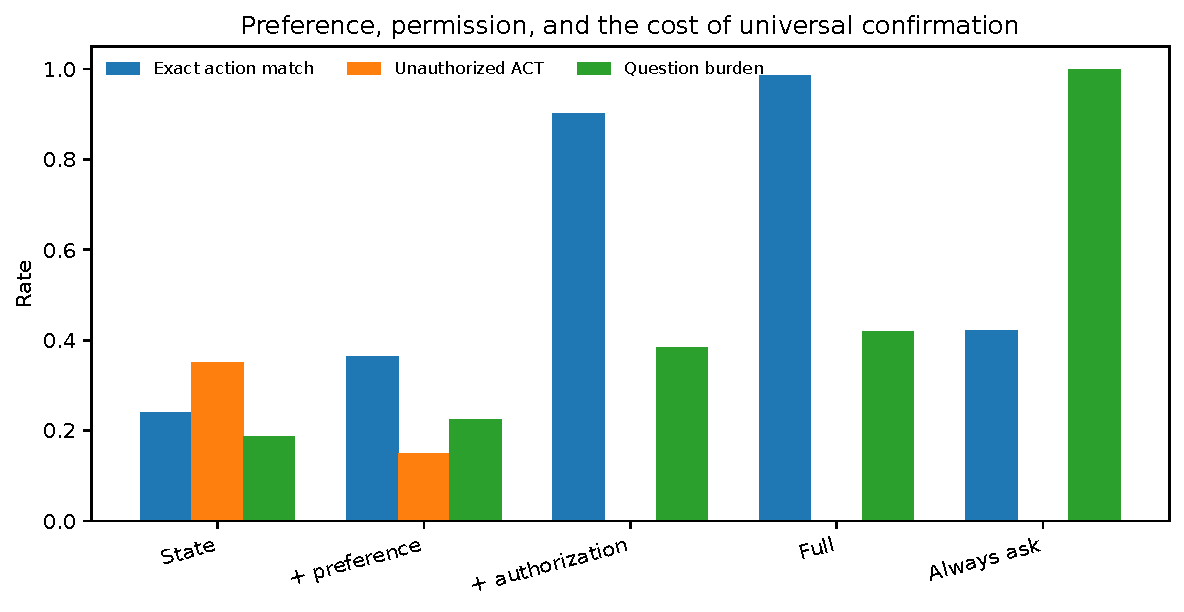
\includegraphics[width=\columnwidth]{figures/factorial_tradeoffs.pdf}
\caption{Synthetic trade-offs. Exact-match strength should not be interpreted as real-world model quality; the main signal is that safety can be ``solved'' trivially by asking constantly, hence burden must be measured.}
\label{fig:tradeoff}
\end{figure}

\subsection{Surface-form stress test}
The strongest canonical number is also the clearest warning against overclaiming. When we evaluate C3 on an unseen paraphrase realization of the same 75 held-out base states, exact match falls from 98.7\% to 52.8\%, acceptable-action rate falls to 76.2\%, and question burden rises to 86.1\% (Figure~\ref{fig:surface}). Unauthorized ACT remains 0\%, suggesting that explicit permission language is still recognized conservatively while finer action selection is brittle. This failure is useful: it demonstrates that the classical baseline exploits surface regularities and that external validation must use semantically varied prompts and stronger models.

\begin{figure}[t]
\centering
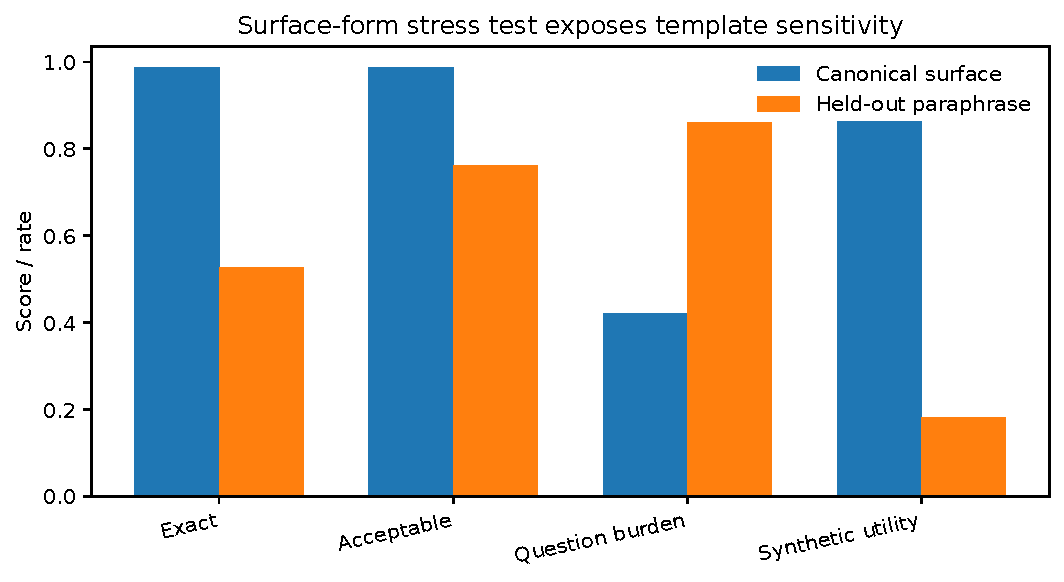
\includegraphics[width=\columnwidth]{figures/surface_generalization.pdf}
\caption{Held-out surface-form stress test. Strong canonical accuracy is not robust to unseen paraphrases.}
\label{fig:surface}
\end{figure}

\subsection{Evidence controls and surface augmentation}
We test whether the canonical C3 result actually depends on the two evidence channels we claim to study. Shuffling authorization statements across held-out scenarios reduces exact match from 98.7\% to 37.6\% and introduces 4.8\% unauthorized autonomous action; masking authorization yields 44.7\% exact and 4.0\% unauthorized action. In contrast, shuffling preference history reduces exact match to 88.6\% while preserving 0\% unauthorized ACT. These controls support a narrower interpretation: authorization language drives boundary compliance in the synthetic pilot, while preference history primarily refines action choice within that boundary (Figure~\ref{fig:controls}).

\begin{figure}[t]
\centering
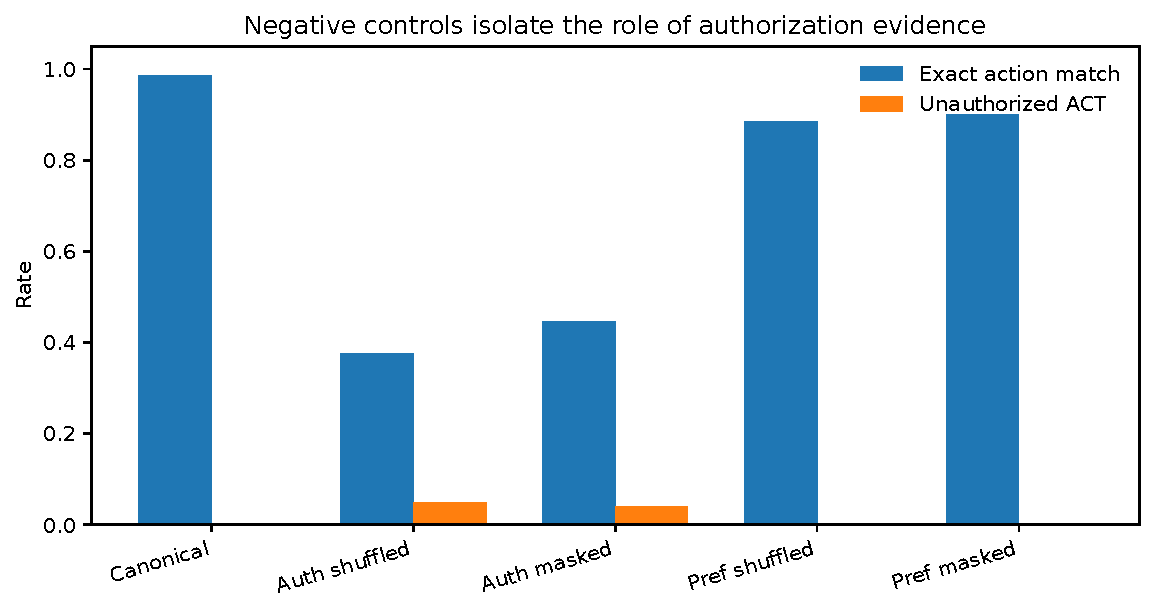
\includegraphics[width=\columnwidth]{figures/evidence_controls.pdf}
\caption{Negative controls. Corrupting authorization evidence sharply reduces exact match and reintroduces unauthorized autonomous action; corrupting preference evidence has a smaller effect on permission compliance.}
\label{fig:controls}
\end{figure}

The paraphrase failure is also partially diagnostic rather than irreducible. Training on a second deterministic surface realization for the \emph{training base states only} raises held-out paraphrase exact match from 52.8\% to 99.0\%, while canonical exact remains 99.1\% (Figure~\ref{fig:aug}). Because both surfaces are still synthetic, this is not evidence of open-ended linguistic robustness. It does show that the observed collapse is largely a surface-coverage problem for this classical text baseline, and motivates semantically diverse external prompts rather than a claim that the intervention formulation itself fails under paraphrase.

\begin{figure}[t]
\centering
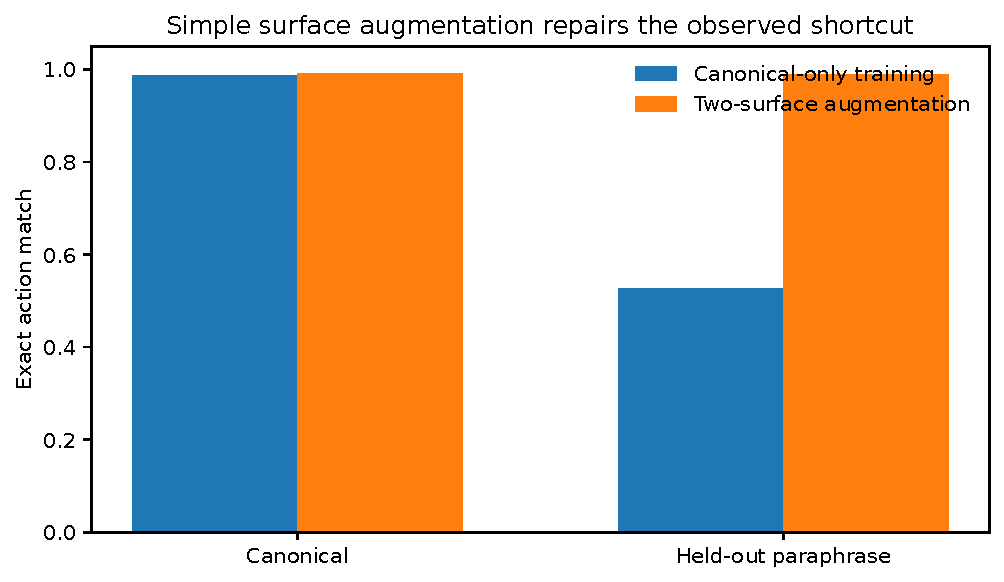
\includegraphics[width=\columnwidth]{figures/surface_augmentation.pdf}
\caption{Surface augmentation. Adding a second training realization for train-only base states repairs most of the held-out paraphrase failure in the synthetic pilot.}
\label{fig:aug}
\end{figure}

\paragraph{Train-subsample and domain robustness.} Across five fits using independent 90\% subsets of the training base states, C3 exact match is 98.56\% $\pm$ 0.08 percentage points (sample standard deviation), with 0\% unauthorized ACT in every run. Leave-one-domain-out training yields 93.1--96.9\% exact across the seven task families. These small variances are reassuring for the deterministic pilot but should not be confused with model-family robustness or human generalization.

\subsection{Utility sensitivity}
We sweep ask cost in $\{0,0.1,0.25,0.5,1.0\}$ and unauthorized-ACT penalty in $\{1,2,3,5,10\}$. C3 has the highest synthetic utility among C3, always-ask, always-silent, and always-suggest in all 25 grid points. This does not validate the utility function; it only shows that the ranking against trivial baselines is not an artifact of the default ask penalty. Human utility weights remain an empirical question.

\subsection{Long-horizon preference drift}
A 100-turn simulator changes the user's synthetic preference at turn 40. A frozen profile overreaches on all post-drift turns; an adaptive profile makes one correction and has 1.7\% post-drift overreach with one-turn adaptation latency (Figure~\ref{fig:drift}). This is a unit-level mechanism test rather than evidence about real human drift.

\begin{figure}[t]
\centering
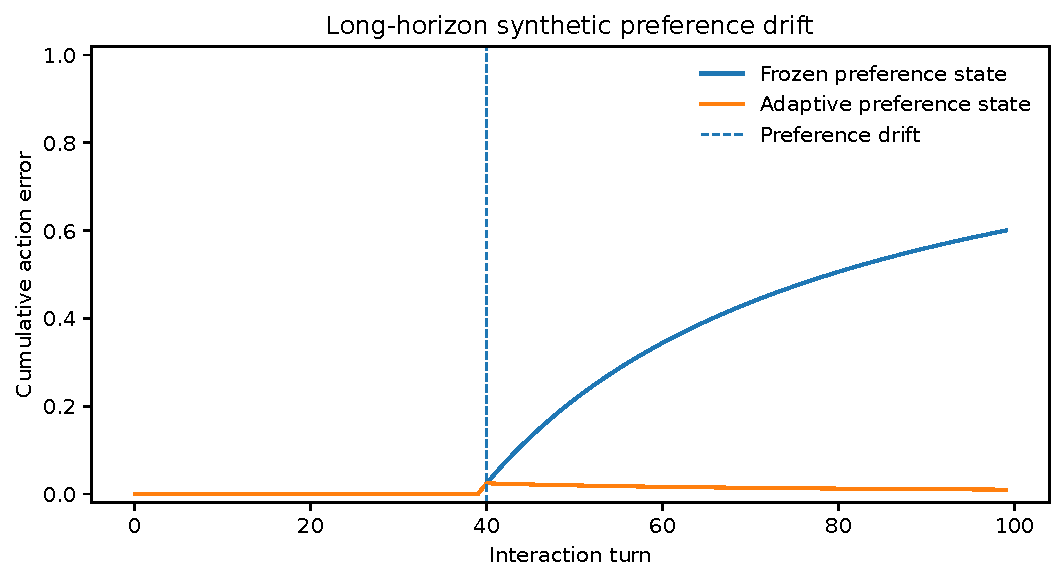
\includegraphics[width=\columnwidth]{figures/long_horizon_drift.pdf}
\caption{Synthetic preference drift. Frozen user state accumulates error after the change point; an explicitly corrected state adapts immediately.}
\label{fig:drift}
\end{figure}


\section{Trajectory-Level Agent Evaluation}
The factorial benchmark isolates intervention judgment, but a deployed agent acts over multiple turns and changes state. We therefore add a small executable harness that represents each evaluation as a task, repeated trials, a full trajectory, multiple graders, and a verified environment outcome. This follows the general agent-evaluation principle that a completion claim in the transcript is not equivalent to success in world state \citep{anthropic2026evals}.

The sandbox contains 144 tasks across six domains (email, calendar, travel, shopping, files, and communication). Authorization takes four values and preference takes three values; selected shopping/file tasks are intentionally irreversible. Each task is run five times for four policy adapters, yielding 2,880 recorded trials. Graders independently check authorization compliance, end-state correctness, interaction efficiency, and recovery behavior. Ask-required recoverable tasks require ask$\rightarrow$confirm$\rightarrow$act; ask-required irreversible tasks require ask$\rightarrow$defer/escalate rather than autonomous mutation.

\begin{table}[t]
\centering\small
\caption{Synthetic trajectory sandbox. pass$^5$ exposes consistency across five trials; it is stricter than pass@1.}
\begin{tabular}{lrrrr}
\toprule
Policy & pass@1 & pass$^5$ & Auth. pass & Recovery \\
\midrule
Preference only & 43.1 & 1.5 & 73.6 & 0.0 \\
Always ask & 91.7 & 64.7 & 91.7 & 83.3 \\
Auth-first + 8\% noise & 96.5 & 83.8 & 99.4 & 91.1 \\
Authorization first & 100.0 & 100.0 & 100.0 & 100.0 \\
\bottomrule
\end{tabular}
\label{tab:trajectory}
\end{table}

\begin{figure}[t]
\centering
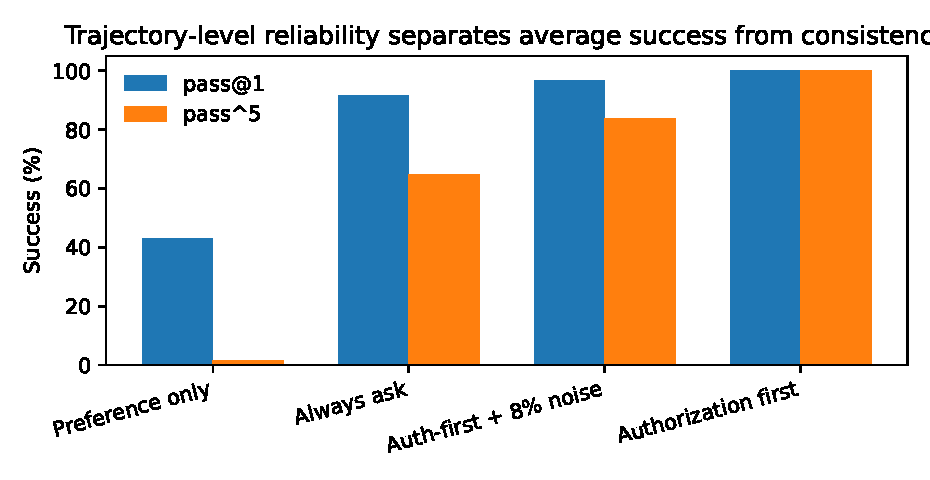
\includegraphics[width=\columnwidth]{figures/trajectory_reliability.pdf}
\caption{Repeated-trial reliability in the executable sandbox. An 8\% seeded action-noise wrapper leaves first-trial performance high but lowers all-five-trials consistency.}
\label{fig:trajectory}
\end{figure}

The harness also turns failed trials into a reproducible incident bank. In the executed run it mined 1,142 incidents and exported the same number of weighted chosen/rejected training records. Authorization overreach is given the highest priority because it has both the largest severity weight and a substantial observed frequency. This closes an executable loop from eval $\rightarrow$ failure taxonomy $\rightarrow$ prioritized data, without claiming that a frontier model was post-trained locally.

\begin{figure}[t]
\centering
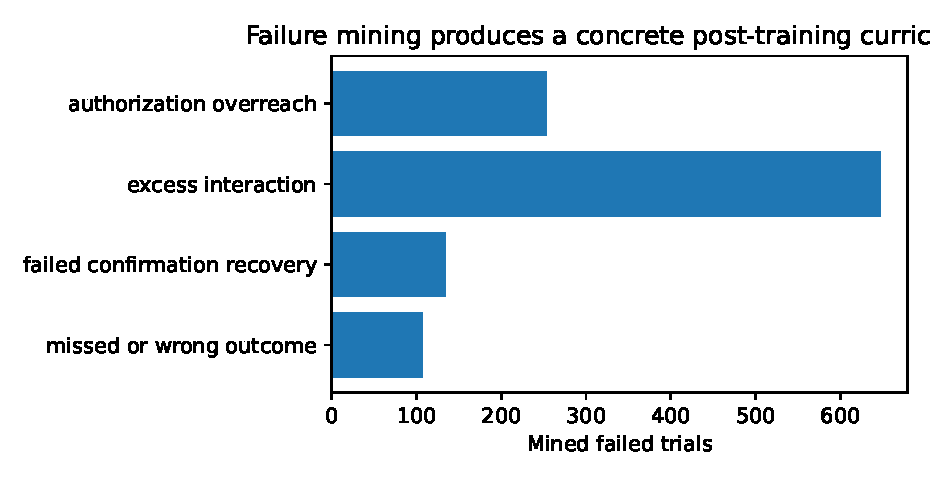
\includegraphics[width=\columnwidth]{figures/incident_mining.pdf}
\caption{Failures mined from recorded trajectories. The release exports both the incident bank and preference-training records for downstream post-training experiments.}
\label{fig:incidents}
\end{figure}


\subsection{Environment shifts and state tracking}
Rule compliance at initialization is not enough for an agent that operates while the environment changes. We therefore add a 90-task shift suite covering matched standard controls plus delayed confirmation, transient pre-mutation tool failure, and permission revocation after confirmation. Each policy is run five times, yielding 1,350 trials across three adapters. The static authorization-first policy passes 80.0\% overall but fails every delayed-confirmation task because it repeatedly asks instead of waiting for the pending response. A state-tracking variant reaches 100\% in the deterministic sandbox by explicitly representing pending confirmation, the latest authorization state, and whether a failed tool call changed external state. With 8\% seeded action noise, pass@1 remains 90.7\% while pass$^5$ falls to 61.3\%, again separating first-run capability from repeated-run reliability.

\begin{table}[t]
\centering\small
\caption{Controlled environment-shift sandbox. ``Tracking'' is a dedicated grader for following the latest environment state.}
\begin{tabular}{lrrrr}
\toprule
Policy & Pass & Auth. pass & Tracking & pass$^5$ \\
\midrule
Authorization first & 80.0 & 100.0 & 66.7 & 32.8 \\
Robust authorization first & 100.0 & 100.0 & 100.0 & 100.0 \\
Robust + 8\% noise & 90.7 & 98.4 & 92.2 & 61.3 \\
\bottomrule
\end{tabular}
\label{tab:shift}
\end{table}

\begin{figure}[t]
\centering
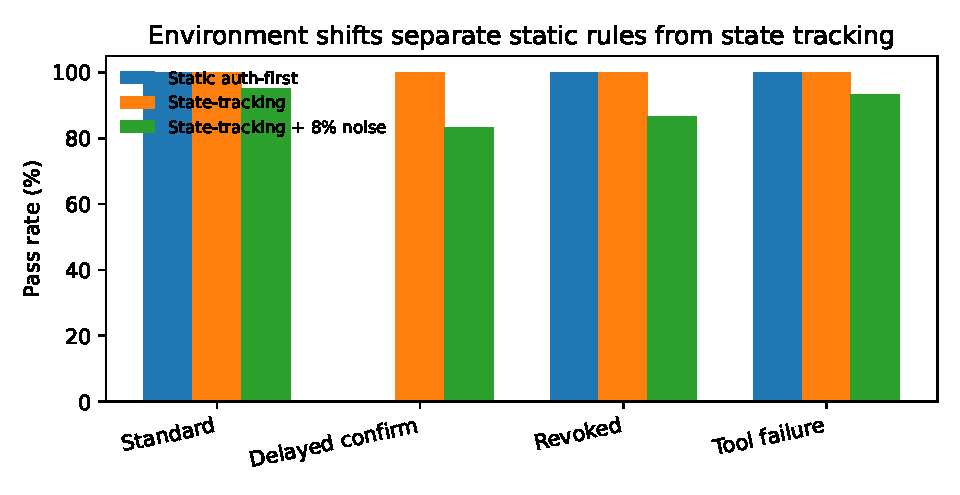
\includegraphics[width=\columnwidth]{figures/cross_environment_reliability.pdf}
\caption{Controlled environment shifts. The static authorization-first policy fails delayed confirmation because it repeats the request instead of representing a pending response.}
\label{fig:crossenv}
\end{figure}

The shift suite is deliberately small and mechanistic. Its role is to catch a class of agent bugs that a static decision benchmark cannot: repeating a request while a confirmation is pending, acting after permission changes, or failing to distinguish a transient pre-mutation tool error from a completed side effect. We also include eleven hand-authored grader-rubric regression cases; all eleven match the expected authorization, outcome, recovery, and state-tracking labels in the release. This is rubric regression, not human grader calibration.

\subsection{Claim-to-evidence gating}
To reduce presentation drift, the release contains a machine-readable registry linking each public research claim to the exact executed artifacts that support it. The audit fails if required evidence is missing. The same registry marks claims that still require human or frontier-model validation and explicitly excludes claims of frontier-model state of the art, human preference validity, deployment safety, or successful production post-training. This does not make the evidence stronger; it makes its scope inspectable.

\section{External Validation Plan}
The publication claim that matters cannot be established by the synthetic oracle. The release therefore makes the missing experiments executable instead of filling them with simulated numbers.

\paragraph{Human validation.} We specify a within-subject factorial study in which participants judge matched preference $\times$ authorization variants. Primary outcomes are authorization violation, appropriateness, helpfulness, perceived control, annoyance, preferred action, and acceptable-action set. The analysis plan uses mixed-effects logistic/ordinal models with participant and base-scenario random effects, reports preregistered contrasts and 95\% confidence intervals, and measures disagreement via Krippendorff's $\alpha$ and label entropy. A simple two-proportion approximation suggests roughly 325 observations per condition for detecting a reduction from 15\% to 8\% at 80\% power; final preregistration should use pilot-based mixed-effects simulation.

\paragraph{Frontier models.} We export 6,000 blinded prompts and define a provider-neutral output schema: scenario id, action, confidence, optional rationale. The scorer computes all protocol metrics without provider-specific code. No frontier-model outputs are included here.

\paragraph{Existing benchmark audit.} The strongest external test is to transform realistic tasks from interactive benchmarks such as KnowU-Bench or long-session corpora such as ProAgentBench into matched permission counterfactuals, subject to licensing and task semantics. A useful result would be that aggregate benchmark performance remains high while counterfactual permission compliance degrades.

\section{Limitations and Safety}
The current numerical evidence is synthetic. The label oracle encodes author choices about what constitutes appropriate intervention. Even after removing structured latent fields, natural-language templates still leak regularities, as the paraphrase failure demonstrates. The classical baseline is not an LLM agent, executes no tools, and does not infer authorization from genuinely ambiguous real-world dialogue. The consequence simulator is schematic. The long-horizon environment contains an explicit correction event rather than naturally learned user-state transitions.

These limitations constrain the claims: we do not conclude that contemporary frontier models exhibit the measured rates, that users agree with the synthetic gold, or that the policy is safe for deployment. High-stakes real actions should require explicit scope, reversible execution where possible, outcome verification, and human escalation. Human and external-model studies must be completed before a strong empirical submission can make population-level claims.

\section{Reproducibility}
The repository includes deterministic data generation, grouped splits, tests, a release audit, exact configs, Croissant metadata, dataset/model cards, and scripts for every table/figure. On the measured release container, the publication-facing v2 block (data generation, C0--C3 evaluation, paraphrase stress test, 100-turn drift) used no GPU, peaked at 206,320 KB resident memory, and ran in 6.71 seconds on 5 visible logical CPUs. The default text baseline uses TF--IDF 1--2 grams (30k feature cap, min df 2) and balanced multinomial logistic regression (max 1000 iterations). External API compute is excluded because it was not executed.

\section{Conclusion}
Personalization and authorization answer different questions. Preference evidence can say what a user tends to want; it does not, by itself, say what an agent is allowed to do now. \system{} turns that distinction into a counterfactual evaluation protocol and makes trivial safety strategies visible through burden and missed-opportunity metrics. The synthetic pilot verifies the mechanics but also reveals substantial template sensitivity. The next scientific step is therefore not another synthetic leaderboard score: it is human validation and frontier-agent auditing under matched preference--permission counterfactuals.

\bibliographystyle{plainnat}
\bibliography{../references}

\appendix
\section{Metric definitions}
For predictions $\hat a_i$ and synthetic gold $g_i$, unauthorized-ACT rate is
\[
\frac{1}{N}\sum_i \mathbf{1}[\hat a_i=\text{act}\wedge z_i\neq\text{preauthorized}].
\]
Question burden is $N^{-1}\sum_i\mathbf{1}[\hat a_i=\text{ask}]$. Unnecessary intervention counts intervention actions when the preferred synthetic action is do-nothing; missed opportunity counts do-nothing when the preferred action is an intervention. Acceptable-action match uses a set-valued synthetic label and is reported separately from exact match.

\section{Hyperparameters and split details}
Generation seeds are 106 (canonical surface), 907 (paraphrase surface), and 19 (group split). The 500 base states yield 4,200/900/900 train/dev/test examples because all twelve counterfactual variants stay with their base state. Full settings are in \texttt{configs/submission\_experiments.yaml}.

\section{Human-study analysis plan}
The preregistration-ready protocol defines authorization violation as the primary binary outcome and appropriateness/control/annoyance as ordinal outcomes. Models include participant and base-scenario random intercepts, with fixed effects for preference condition, authorization, stakes, reversibility, and preregistered interactions. Individual-level judgments remain distinct from consensus labels so personalization is not erased by aggregation.

\section{Artifact status}
The archive contains executed synthetic results and unexecuted external-evidence harnesses. Files under \texttt{frontier\_eval/} export prompts and score predictions; \texttt{human\_study/} contains blinded annotation items, schema, protocol, and power-analysis tooling. The paper deliberately leaves external result cells absent rather than populating them with fabricated model or participant outputs.
\end{document}
